% Template created by Robert Maier, 2013
\documentclass[t,plaincaption]{beamer}

\mode<presentation>
{
	\usepackage{theme_cvpr/beamerthemeCVPR}
	\setbeamercovered{transparent}
}

\usepackage{verbatim}

% Use xelatex to use TTF fonts 
\usepackage{fontspec}
\setsansfont{Arial}

% set the bibliography style
%\bibliographystyle{abbrv}
\bibliographystyle{apalike}

% set document information
\def\titleEn{Random GP Forest}
\def\authorName{Raphael Dümig, Andreas Wiedemann, Nan Liu, Dragomir Nikolic\\
\vspace{0.5cm}
Supervisor: Dr. habil. Rudolph Triebel}
\title[\titleEn]{\titleEn}
\author[Raphael Dümig, Andreas Wiedemann, Nan Liu, Dragomir Nikolic: \titleEn]{\authorName}
\date{July 27, 2015}


\begin{document}

\frame{
\titlepage 
}

\frame{
\frametitle{Outline}

\tableofcontents
}


\section{Problem}
\frame{
\frametitle{Problem}

\begin{columns}[t]
\begin{column}{0.45\linewidth}
\begin{itemize}
\item Gaussian Process (GP)
\begin{itemize}
\item high training time complexity	
\end{itemize}
\vspace{0.5cm}
\item Random Forest (RDF)
\begin{itemize}
\item 	moderate accuracy rate
\end{itemize}
%\vspace{0.5cm}
\end{itemize}
\end{column}

\begin{column}{0.65\linewidth}
\begin{figure}[t]
\centering

\begin{center}
\hspace{-3cm}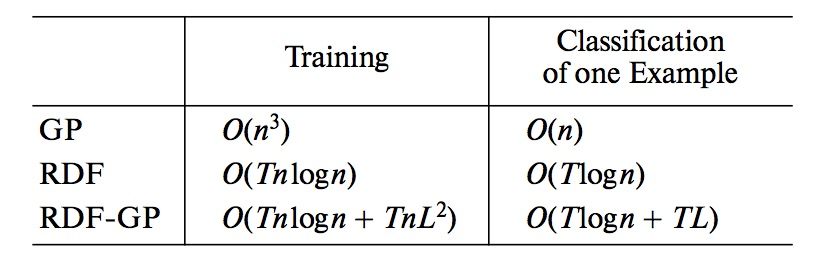
\includegraphics[width=3cm,height=1cm]{time}
\end{center}
\vspace{0.3cm}
\scriptsize{Table 1: Computational complexity: n denotes the number of training examples, L refers to the maximum number of examples a GP classifier is learned within a leaf, T is the number of decision trees in the forest$_{[1]}$.}

\end{figure}
\end{column}
\end{columns}
}


\section{Objective}
\frame{
\frametitle{Objective}

\begin{columns}[t]
\begin{column}{0.5\linewidth}
\begin{itemize}
\item Combining RDF and GP (RDF-GP)
\begin{itemize}
\item enable accurate classification in large-scale settings
\item GP: state-of-the-art recognition performance
\item RDF:  applied to large-scale dataset
\end{itemize}
\end{itemize}
\end{column}

\begin{column}{0.5\linewidth}
\begin{figure}[t]
\centering
\hspace{-2.5cm}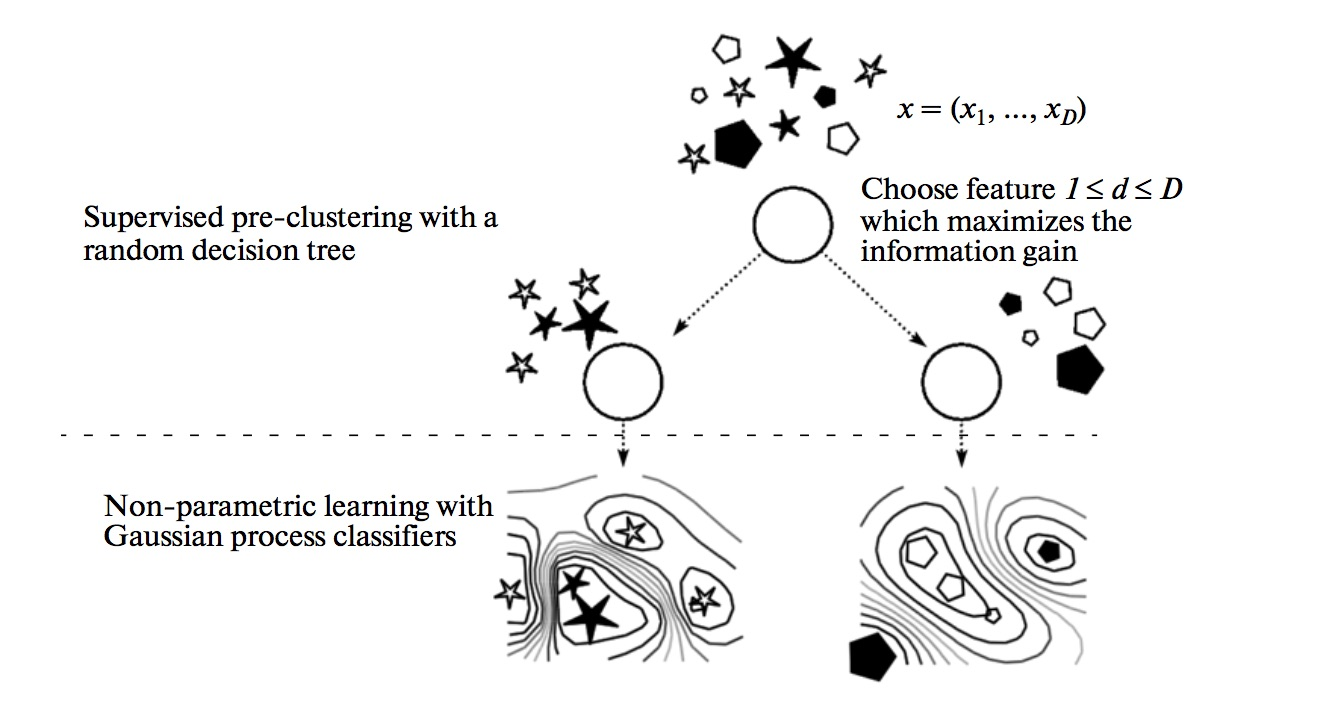
\includegraphics[width=0.5\linewidth]{fig1}

%\vspace{0.5cm}
\scriptsize{Figure 1: RDF is used to cluster the data in a supervised manner and a GP classifier is used to separate classes in each leaf$_{[1]}$.}
\label{fig1}
\end{figure}
\end{column}
\end{columns}
}

\section{Implementation}

\frame{
\frametitle{Implementation}

\begin{itemize}
	\item GP [Raphael Dümig, Dragomir Nikolic]
	\begin{itemize}
		\item library: GPc by Neil Lawrence$_{[4]}$
		\item challenges:
		\begin{itemize}
			\item IVM supports online learning but does not accept single samples
			\item training data with samples from a single class creates exceptions
			\item IVM performs only a binary classification
		\end{itemize}
		\item solutions:
		\begin{itemize}
			\item buffer samples until there are enough samples
			\item buffer samples until they belong to more than one class
			\item train a separate IVM for each class
		\end{itemize}
	\end{itemize}
\end{itemize}

}

\frame{
\frametitle{Implementation}

\begin{itemize}
\item  RDF [Andreas Wiedemann, Nan Liu]
\begin{itemize}
\item OpenCV library\ \ \ \ off-line version
\item Amir Saffari [3]\ \ \ \ \ on-line version
\end{itemize}
\end{itemize}
}
\frame{
\frametitle{Implementation}
\begin{columns}[t]
\begin{column}{0.5\linewidth}
\begin{figure}[t]
\centering
\vspace{2cm}
\hspace{-2cm}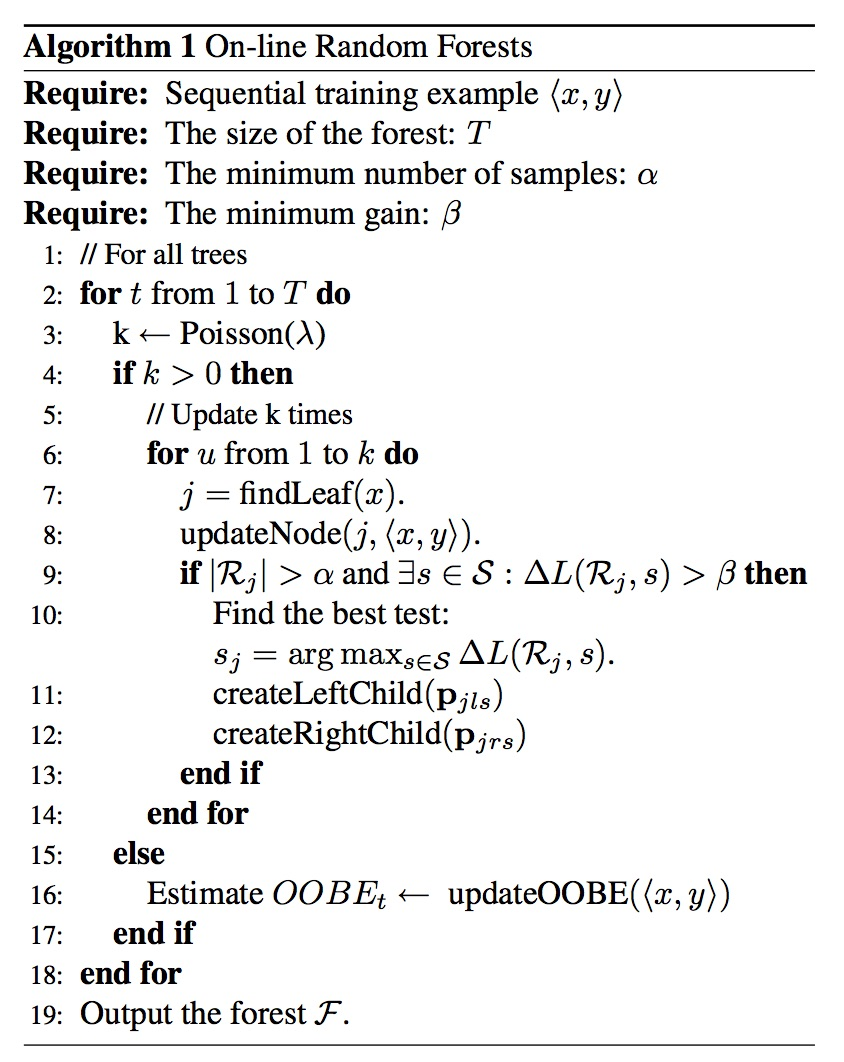
\includegraphics[width=2cm,height=3cm]{rdfalg}

\scriptsize{Figure 2: Online RDF algorithm$_{[3]}$.}
\label{fig2}
\end{figure}
\end{column}

\begin{column}{0.5\linewidth}
\begin{figure}[t]
\centering
\vspace{2cm}
\hspace{-2.8cm}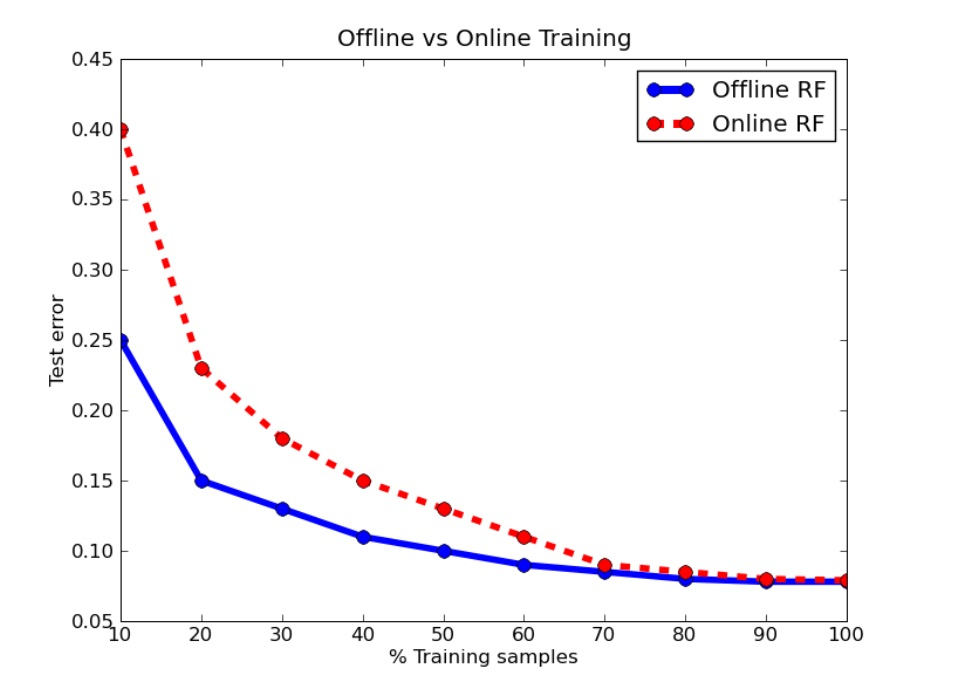
\includegraphics[width=3cm,height=1.5cm]{rdf_perf_onoff}

\scriptsize{Figure 3: Classification error with respect to the ratio of labeled samples for off-line and on-line training with increasing number of training samples$_{[3]}$.}
\label{fig3}
\end{figure}
\end{column}
\end{columns}

}


%\section{Implementation}
\frame{
\frametitle{Implementation}

\begin{itemize}
\item Combining GP with online RDF
\begin{itemize}
\item Challenge 1:  when to train GP?
\item Solution:  buffer
\item Challenge 2:  multiclassification?
\item Solution:  train n GPCs for each leaf node
\end{itemize}
\end{itemize}
}

\section{Milestones}
\frame{
\frametitle{Milestones}

\begin{figure}[t]
\centering
\vspace{2cm}
\hspace{-3.8cm}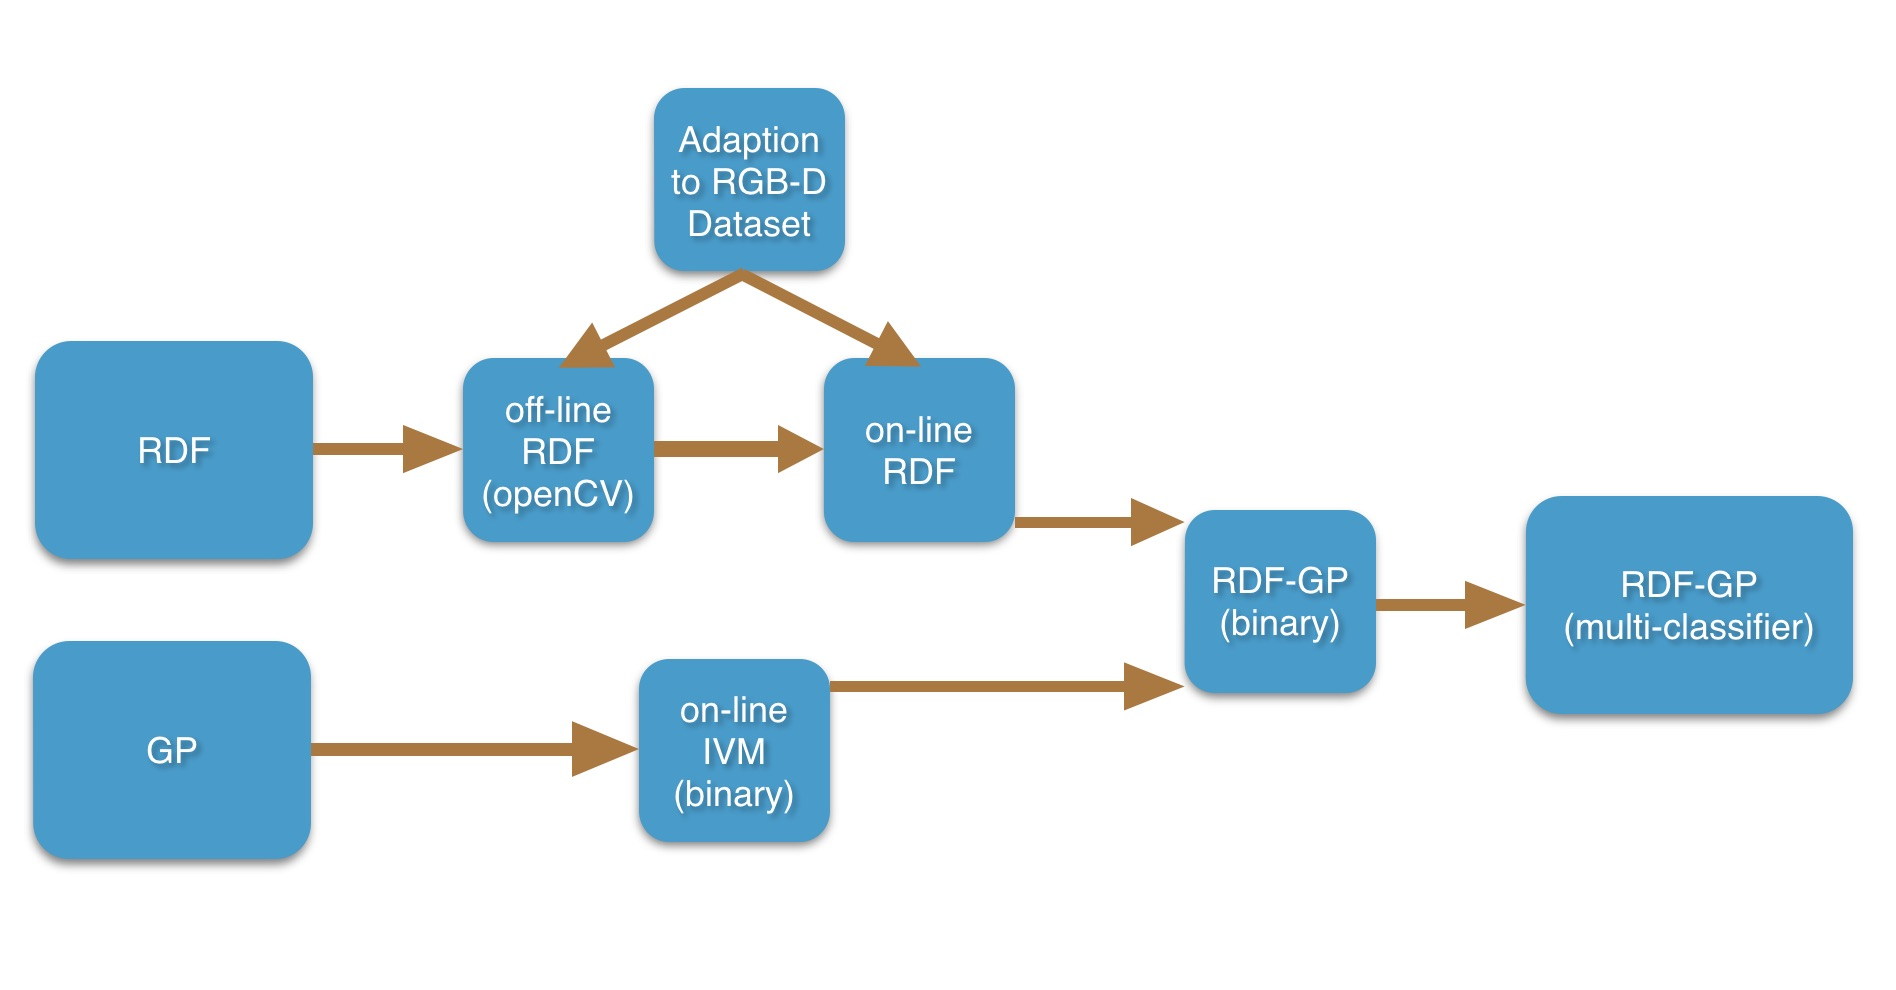
\includegraphics[width=4.5cm,height=2.7cm]{andi}

\scriptsize{Figure 4: Online RDF algorithm.}
\label{fig4}
\end{figure}
}


\section{Experiments and Evaluation}
\frame{
\frametitle{Experiments and Evaluation}
\begin{itemize}
\item Data: RGB-D Dataset$_{[2]}$ 
\end{itemize}

\begin{figure}
	\centering
	\begin{minipage}{0.45\textwidth}
		\centering
		% GNUPLOT: LaTeX picture
\setlength{\unitlength}{0.240900pt}
\ifx\plotpoint\undefined\newsavebox{\plotpoint}\fi
\sbox{\plotpoint}{\rule[-0.200pt]{0.400pt}{0.400pt}}%
\begin{picture}(1181,590)(0,0)
\sbox{\plotpoint}{\rule[-0.200pt]{0.400pt}{0.400pt}}%
\put(110.0,82.0){\rule[-0.200pt]{4.818pt}{0.400pt}}
\put(90,82){\makebox(0,0)[r]{$0$}}
\put(1100.0,82.0){\rule[-0.200pt]{4.818pt}{0.400pt}}
\put(110.0,159.0){\rule[-0.200pt]{4.818pt}{0.400pt}}
\put(90,159){\makebox(0,0)[r]{$0.2$}}
\put(1100.0,159.0){\rule[-0.200pt]{4.818pt}{0.400pt}}
\put(110.0,236.0){\rule[-0.200pt]{4.818pt}{0.400pt}}
\put(90,236){\makebox(0,0)[r]{$0.4$}}
\put(1100.0,236.0){\rule[-0.200pt]{4.818pt}{0.400pt}}
\put(110.0,312.0){\rule[-0.200pt]{4.818pt}{0.400pt}}
\put(90,312){\makebox(0,0)[r]{$0.6$}}
\put(1100.0,312.0){\rule[-0.200pt]{4.818pt}{0.400pt}}
\put(110.0,389.0){\rule[-0.200pt]{4.818pt}{0.400pt}}
\put(90,389){\makebox(0,0)[r]{$0.8$}}
\put(1100.0,389.0){\rule[-0.200pt]{4.818pt}{0.400pt}}
\put(110.0,466.0){\rule[-0.200pt]{4.818pt}{0.400pt}}
\put(90,466){\makebox(0,0)[r]{$1$}}
\put(1100.0,466.0){\rule[-0.200pt]{4.818pt}{0.400pt}}
\put(278.0,82.0){\rule[-0.200pt]{0.400pt}{4.818pt}}
\put(278,41){\makebox(0,0){RDF}}
\put(278.0,446.0){\rule[-0.200pt]{0.400pt}{4.818pt}}
\put(615.0,82.0){\rule[-0.200pt]{0.400pt}{4.818pt}}
\put(615,41){\makebox(0,0){RDF-GP}}
\put(615.0,446.0){\rule[-0.200pt]{0.400pt}{4.818pt}}
\put(952.0,82.0){\rule[-0.200pt]{0.400pt}{4.818pt}}
\put(952,41){\makebox(0,0){GP}}
\put(952.0,446.0){\rule[-0.200pt]{0.400pt}{4.818pt}}
\put(110.0,82.0){\rule[-0.200pt]{0.400pt}{92.506pt}}
\put(110.0,82.0){\rule[-0.200pt]{243.309pt}{0.400pt}}
\put(1120.0,82.0){\rule[-0.200pt]{0.400pt}{92.506pt}}
\put(110.0,466.0){\rule[-0.200pt]{243.309pt}{0.400pt}}
\put(615,528){\makebox(0,0){Accuracies of classifiers}}
\put(194,82){\rule{40.953pt}{30.8352pt}}
\put(194.0,82.0){\rule[-0.200pt]{0.400pt}{30.594pt}}
\put(194.0,209.0){\rule[-0.200pt]{40.712pt}{0.400pt}}
\put(363.0,82.0){\rule[-0.200pt]{0.400pt}{30.594pt}}
\put(531,82){\rule{40.7121pt}{47.4573pt}}
\put(194.0,82.0){\rule[-0.200pt]{40.712pt}{0.400pt}}
\put(531.0,82.0){\rule[-0.200pt]{0.400pt}{47.216pt}}
\put(531.0,278.0){\rule[-0.200pt]{40.471pt}{0.400pt}}
\put(699.0,82.0){\rule[-0.200pt]{0.400pt}{47.216pt}}
\put(868,82){\rule{40.7121pt}{65.043pt}}
\put(531.0,82.0){\rule[-0.200pt]{40.471pt}{0.400pt}}
\put(868.0,82.0){\rule[-0.200pt]{0.400pt}{64.802pt}}
\put(868.0,351.0){\rule[-0.200pt]{40.471pt}{0.400pt}}
\put(1036.0,82.0){\rule[-0.200pt]{0.400pt}{64.802pt}}
\put(868.0,82.0){\rule[-0.200pt]{40.471pt}{0.400pt}}
\put(110.0,82.0){\rule[-0.200pt]{0.400pt}{92.506pt}}
\put(110.0,82.0){\rule[-0.200pt]{243.309pt}{0.400pt}}
\put(1120.0,82.0){\rule[-0.200pt]{0.400pt}{92.506pt}}
\put(110.0,466.0){\rule[-0.200pt]{243.309pt}{0.400pt}}
\end{picture}

	\end{minipage}
	\hfill
	\begin{minipage}{0.45\textwidth}
		\centering
		% GNUPLOT: LaTeX picture
\setlength{\unitlength}{0.240900pt}
\ifx\plotpoint\undefined\newsavebox{\plotpoint}\fi
\sbox{\plotpoint}{\rule[-0.200pt]{0.400pt}{0.400pt}}%
\begin{picture}(708,531)(0,0)
\sbox{\plotpoint}{\rule[-0.200pt]{0.400pt}{0.400pt}}%
\put(130.0,82.0){\rule[-0.200pt]{4.818pt}{0.400pt}}
\put(110,82){\makebox(0,0)[r]{$0$}}
\put(627.0,82.0){\rule[-0.200pt]{4.818pt}{0.400pt}}
\put(130.0,128.0){\rule[-0.200pt]{4.818pt}{0.400pt}}
\put(110,128){\makebox(0,0)[r]{$200$}}
\put(627.0,128.0){\rule[-0.200pt]{4.818pt}{0.400pt}}
\put(130.0,175.0){\rule[-0.200pt]{4.818pt}{0.400pt}}
\put(110,175){\makebox(0,0)[r]{$400$}}
\put(627.0,175.0){\rule[-0.200pt]{4.818pt}{0.400pt}}
\put(130.0,221.0){\rule[-0.200pt]{4.818pt}{0.400pt}}
\put(110,221){\makebox(0,0)[r]{$600$}}
\put(627.0,221.0){\rule[-0.200pt]{4.818pt}{0.400pt}}
\put(130.0,268.0){\rule[-0.200pt]{4.818pt}{0.400pt}}
\put(110,268){\makebox(0,0)[r]{$800$}}
\put(627.0,268.0){\rule[-0.200pt]{4.818pt}{0.400pt}}
\put(130.0,314.0){\rule[-0.200pt]{4.818pt}{0.400pt}}
\put(110,314){\makebox(0,0)[r]{$1000$}}
\put(627.0,314.0){\rule[-0.200pt]{4.818pt}{0.400pt}}
\put(130.0,361.0){\rule[-0.200pt]{4.818pt}{0.400pt}}
\put(110,361){\makebox(0,0)[r]{$1200$}}
\put(627.0,361.0){\rule[-0.200pt]{4.818pt}{0.400pt}}
\put(130.0,407.0){\rule[-0.200pt]{4.818pt}{0.400pt}}
\put(110,407){\makebox(0,0)[r]{$1400$}}
\put(627.0,407.0){\rule[-0.200pt]{4.818pt}{0.400pt}}
\put(216.0,82.0){\rule[-0.200pt]{0.400pt}{4.818pt}}
\put(216,41){\makebox(0,0){RDF}}
\put(216.0,387.0){\rule[-0.200pt]{0.400pt}{4.818pt}}
\put(389.0,82.0){\rule[-0.200pt]{0.400pt}{4.818pt}}
\put(389,41){\makebox(0,0){RDF-GP}}
\put(389.0,387.0){\rule[-0.200pt]{0.400pt}{4.818pt}}
\put(561.0,82.0){\rule[-0.200pt]{0.400pt}{4.818pt}}
\put(561,41){\makebox(0,0){GP}}
\put(561.0,387.0){\rule[-0.200pt]{0.400pt}{4.818pt}}
\put(130.0,82.0){\rule[-0.200pt]{0.400pt}{78.292pt}}
\put(130.0,82.0){\rule[-0.200pt]{124.545pt}{0.400pt}}
\put(647.0,82.0){\rule[-0.200pt]{0.400pt}{78.292pt}}
\put(130.0,407.0){\rule[-0.200pt]{124.545pt}{0.400pt}}
\put(388,469){\makebox(0,0){Computation time in $sec$}}
\put(345,82){\rule{21.1992pt}{26.7399pt}}
\put(345.0,82.0){\rule[-0.200pt]{0.400pt}{26.499pt}}
\put(345.0,192.0){\rule[-0.200pt]{20.958pt}{0.400pt}}
\put(432.0,82.0){\rule[-0.200pt]{0.400pt}{26.499pt}}
\put(518,82){\rule{20.9583pt}{72.0291pt}}
\put(345.0,82.0){\rule[-0.200pt]{20.958pt}{0.400pt}}
\put(518.0,82.0){\rule[-0.200pt]{0.400pt}{71.788pt}}
\put(518.0,380.0){\rule[-0.200pt]{20.717pt}{0.400pt}}
\put(604.0,82.0){\rule[-0.200pt]{0.400pt}{71.788pt}}
\put(518.0,82.0){\rule[-0.200pt]{20.717pt}{0.400pt}}
\put(130.0,82.0){\rule[-0.200pt]{0.400pt}{78.292pt}}
\put(130.0,82.0){\rule[-0.200pt]{124.545pt}{0.400pt}}
\put(647.0,82.0){\rule[-0.200pt]{0.400pt}{78.292pt}}
\put(130.0,407.0){\rule[-0.200pt]{124.545pt}{0.400pt}}
\end{picture}

	\end{minipage}

	\scriptsize{results for 200 training and 100 testing samples}
\end{figure}

}

 
\section{Conclusion and Future Work}
\frame{
\frametitle{Conclusion and Future Work}

\begin{itemize}
\item Our Contributions:
\begin{itemize}
\item combined GP and RDF
\item implemented online version
\item obtained multi classifier
\end{itemize}
\end{itemize}

\begin{itemize}
\item Advantages:
\begin{itemize}
\item good accuracy maintained
\item substantially faster than the full GP classifier
\end{itemize}
\end{itemize}


\begin{itemize}
\item Future Work:
\begin{itemize}
\item parameter optimization 
\item used for large data set
\item using GPU for speed optimization
\item feature selection (PCA)
\end{itemize}
\end{itemize}

}

\frame[allowframebreaks]{
\frametitle{Bibliography}
	\tiny
	\bibliography{bibliography} 
\begin{thebibliography}{99}
\bibitem{1}
B. Fröhlich, E. Rodner, M. Kemmler, and J. Denzler,	 “Large-Scale Gaussian Process Classification Using Random Decision Forests, ” ISSN 1054-6618, Pattern Recognition and Image Analysis, 2012, Vol. 22, No. 1, pp. 113–120, 2012.

\bibitem{2}
Kevin Lai, Liefeng Bo, Xiaofeng Ren, and Dieter Fox.  A Large-Scale Hierarchical Multi-View RGB-D Object Dataset. http://rgbd-dataset.cs.washington.edu

\bibitem{3}
Amir Saffari, Christian Leistner, Jakob Santner, Martin Godec, and Horst Bischof, "On-line Random Forests," 3rd IEEE ICCV Workshop on On-line Computer Vision, 2009.

\bibitem{4}
Neil Lawrence. Github repository of GPc -- opened on 26. July 2015: https://github.com/SheffieldML/GPc

\end{thebibliography}
}

\end{document}
